\chapter{Related Work}
\label{chapter:related_work}

\section{Directory Service}
Also known as name service, maps the names of network resources to their respective network addresses. Each resource on the network is considered an object by the directory server. Information about a particular resource is stored as a collection of attributes associated with that resource or object. One of the most representing example is the DNS, which offers internet domain names translation to ip addresses.

\section{DHT and P2P Networks}
A distributed hash table (DHT) is a class of a decentralised distributed system that provides a lookup service similar to a hash table: (key, value) pairs are stored in a DHT, and any participating node can efficiently retrieve the value associated with a given key

\subsection{DHT characteristics}
\begin{list}{}{}
\item \emph{Autonomy and decentralization}: multiple nodes, no central coordinator;
\item \emph{Fault tolerance}: reliable, no single point of failure (like Napster’s central server) (Byzantine fault tolerance);
\item \emph{Scalability}: the system scales. This means it’s working efficiently regardless the workload;
\item \emph{Load balancing} (optional);
\item \emph{Data integrity} (optional).
\end{list}

\subsection{Functioning Example}
Once these components are in place, a typical use of the DHT for storage and retrieval might proceed as follows. Suppose the keyspace is the set of 160-bit strings. To index a file with given filename and data in the DHT, the SHA-1 hash of filename is generated, producing a 160-bit key k, and a message put(k, data) is sent to any node participating in the DHT. The message is forwarded from node to node through the overlay network until it reaches the single node responsible for key k as specified by the keyspace partitioning. That node then stores the key and the data. Any other client can then retrieve the contents of the file by again hashing filename to produce k and asking any DHT node to find the data associated with k with a message get(k). The message will again be routed through the overlay to the node responsible for k, which will reply with the stored data.

\subsection{The Network}
Each node maintains a set of links to other nodes (its neighbors or routing table). Together, these links form the overlay network. A node picks its neighbors according to a certain structure, called the network's topology.

Aside from routing, there exist many algorithms that exploit the structure of the overlay network for sending a message to all nodes, or a subset of nodes, in a DHT. These algorithms are used by applications to do overlay multicast, range queries, or to collect statistic. (Flooding).

\subsection*{Implementations Considered}
\begin{list}{}{}
\item Kademlia
\item TomP2P
\end{list}

\section{Blockchain Implementations}

\subsection*{Blockchain introduction}
Blockchain’s distributed ledger system is used to keep track of Bitcoin transactions. Blockchain eliminates the need for central authorities and enables each user of the system to maintain their own copy of the ledger. It also keeps all copies of the ledger synchronized through a consensus algorithm.Bitcoin miners do the recording and validation of the transactions. The miners are necessary to prevent ‘double spend.’
\subsection*{Bitcoin}
Blockchain is a distributed ledger technology used to keep track of Bitcoin cryptocurrency transactions. Distributed ledgers create a data structure – like a chain – where records of every single Bitcoin transaction live. To prevent “double spend,” all Bitcoin transactions are validated and then permanently archived in the cryptographic ledger or chain. The validation is done via a peer-to-peer process that is hugely computer-intensive. It is supported by a global network of volunteers – known as “miners” – who are incentivized mainly by Bitcoin’s mining reward.
In essence, Bitcoin uses cryptography to enable participants on the network to update the ledger in a secure way without the need for a central authority. The key to Blockchain was to agree on the order of entries in the ledger. Once this was in place, distributed control of Bitcoin was possible.

\subsection*{Namecoin}
Namecoin is an experimental open-source technology which improves decentralization, security, censorship resistance, privacy, and speed of certain components of the Internet infrastructure such as DNS and identities. Namecoin is a key/value pair registration and transfer system based on the Bitcoin technology.
What does Namecoin do under the hood?
\begin{list}{}{}
\item Securely record and transfer arbitrary names (keys).
\item Attach a value (data) to the names (up to 520 bytes).
\item Transact the digital currency namecoins (NMC).
\item Like bitcoins, Namecoin names are difficult to censor or seize.
\item Lookups do not generate network traffic (improves privacy).
\end{list}

\subsection*{Hyperledger / Hyperledger Fabric}
Hyperledger is an open source collaborative effort created to advance cross-industry blockchain technologies. It is a global collaboration, hosted by The Linux Foundation, including leaders in finance, banking, Internet of Things, supply chains, manufacturing and Technology.
Hyperledger Fabric is a business blockchain framework hosted on Hyperledger intended as a foundation for developing blockchain applications or solutions with a modular architecture. Hyperledger Fabric allows components such as consensus and membership services to be plug-and-play.
Hyperledger Fabric establishes trust, transparency, and accountability based on the following principles:
\begin{list}{}{}
\item Permissioned network - Provides collectively defined membership and access rights within your business network
\item Confidential transactions - Gives businesses the flexibility and security to make transactions visible to select parties with the correct encryption keys
\item No cryptocurrency - Does not require mining and expensive computations to assure transactions
\item Programmable - Leverage the embedded logic in smart contracts to automate business processes across your network
\end{list}

\subsection*{Ehtereum}
Ethereum is a  decentralized platform that runs smart contracts: applications that run exactly as programmed without any possibility of downtime, censorship, fraud or third party interference.
These apps run on a custom built  blockchain, an enormously powerful shared global infrastructure that can move value around and represent the ownership of property. This enables developers to create markets, store registries of debts or promises, move funds in accordance with instructions given long in the past (like a will or a futures contract) and many other things that have not been invented yet, all without a middle man or counterparty risk.
On traditional server architectures, every application has to set up its own servers that run their own code in isolated silos, making sharing of data hard. If a single app is compromised or goes offline, many users and other apps are affected.
On a blockchain, anyone can set up a node that replicates the necessary data for all nodes to reach an agreement and be compensated by users and app developers. This allows user data to remain private and apps to be decentralized like the Internet was supposed to work.
\subsection*{Storj}
Storj is a peer-to-peer cloud storage network implementing client-side encryption would allow users to transfer and share data without reliance on a third party storage provider. The removal of central controls would mitigate most traditional data failures and outages, as well as significantly increase security, privacy, and data control. Peer-to-peer networks are generally unfeasible for production storage systems, as data availability is a function of popularity, rather than utility.
\subsection*{Swarm}
Swarm is a distributed storage platform and content distribution service, a native base layer service of the ethereum web 3 stack. The primary objective of Swarm is to provide a decentralized and redundant store of Ethereum's public record, in particular to store and distribute dapp code and data as well as block chain data.
From the end user's perspective, Swarm is not that different from WWW, except that uploads are not to a specific server. The objective is to peer-to-peer storage and serving solution that is DDOS-resistant, zero-downtime, fault-tolerant and censorship-resistant as well as self-sustaining due to a built-in incentive system which uses peer to peer accounting and allows trading resources for payment. Swarm is designed to deeply integrate with the devp2p multiprotocol network layer of Ethereum as well as with the Ethereum blockchain for domain name resolution, service payments and content availability insurance.
\subsection*{IPFS}
The InterPlanetary File System (IPFS) is a peer-to-peer distributed file system that seeks to connect all computing devices with the same system of files. In some ways, IPFS is similar to the Web, but IPFS could be seen as a single BitTorrent swarm, exchanging objects within one Git repository. In other words, IPFS provides a high throughput content-addressed block storage model, with contentaddressed hyper links. This forms a generalized Merkle DAG, a data structure upon which one can build versioned file systems, blockchains, and even a Permanent Web. IPFS combines a distributed hashtable, an incentivized block exchange, and a self-certifying namespace. IPFS has no single point of failure, and nodes do not need to trust each other.
\subsection*{Filecoin}
Filecoin is a distributed electronic currency similar to Bitcoin. Unlike Bitcoin’s computation-only proof-of-work, Filecoin’s proof-of-work function includes a proof-of-retrievability component, which requires nodes to prove they store a particular file. The Filecoin network forms an entirely distributed file sorage system, whose nodes are incentivized to store as much of the entire network’s data as they can. The currency is awarded for storing files, and is transferred in transactions, as in Bitcoin. Files are added to the network by spending currency. This produces strong monetary incentives for individuals to join and work for the network. In the course of ordinary operation of the Filecoin network, nodes contribute useful work in the form of storage and distribution of valuable data.

\subsection*{BigChainDB}

BigChainDB is aiming to merge database and Blockchain, trying to keep all the properties of the first such as a lineat scaling throuhput, an efficient query language and permissions in order to interact with it. In particular developing a MongoDB based NoSQL distributed database.
With the foundamental features of Blockchain as decentralisation, immutability, creation and movement of digital assets.
One interesting approach with BigChainDB is that it can be integrated with Ethereum (sort of its database) and be run on private or public networks.

\section{Blockstack Use Case}
Blockstack is a particular implementation of a decentralized DNS system based on blockchain. It combines DNS functionality with public key infrastructure and is primarily meant to be used by new blockchain applications.

According to the company: \"under the hood, Blockstack provides a decentralized domain name system (DNS), decentralized public key distribution system, and registry for apps and user identities\" [add reference].

The real breakthrough is the architecture the system is built on. It can be described as a three-layer design with the blockchain as the first and lower tier, the storage system as the upper and the peer network as middle layer.

The architecture is shown in \ref{fig:blockstack-architecture}.
\begin{figure}[h]
	\centering
  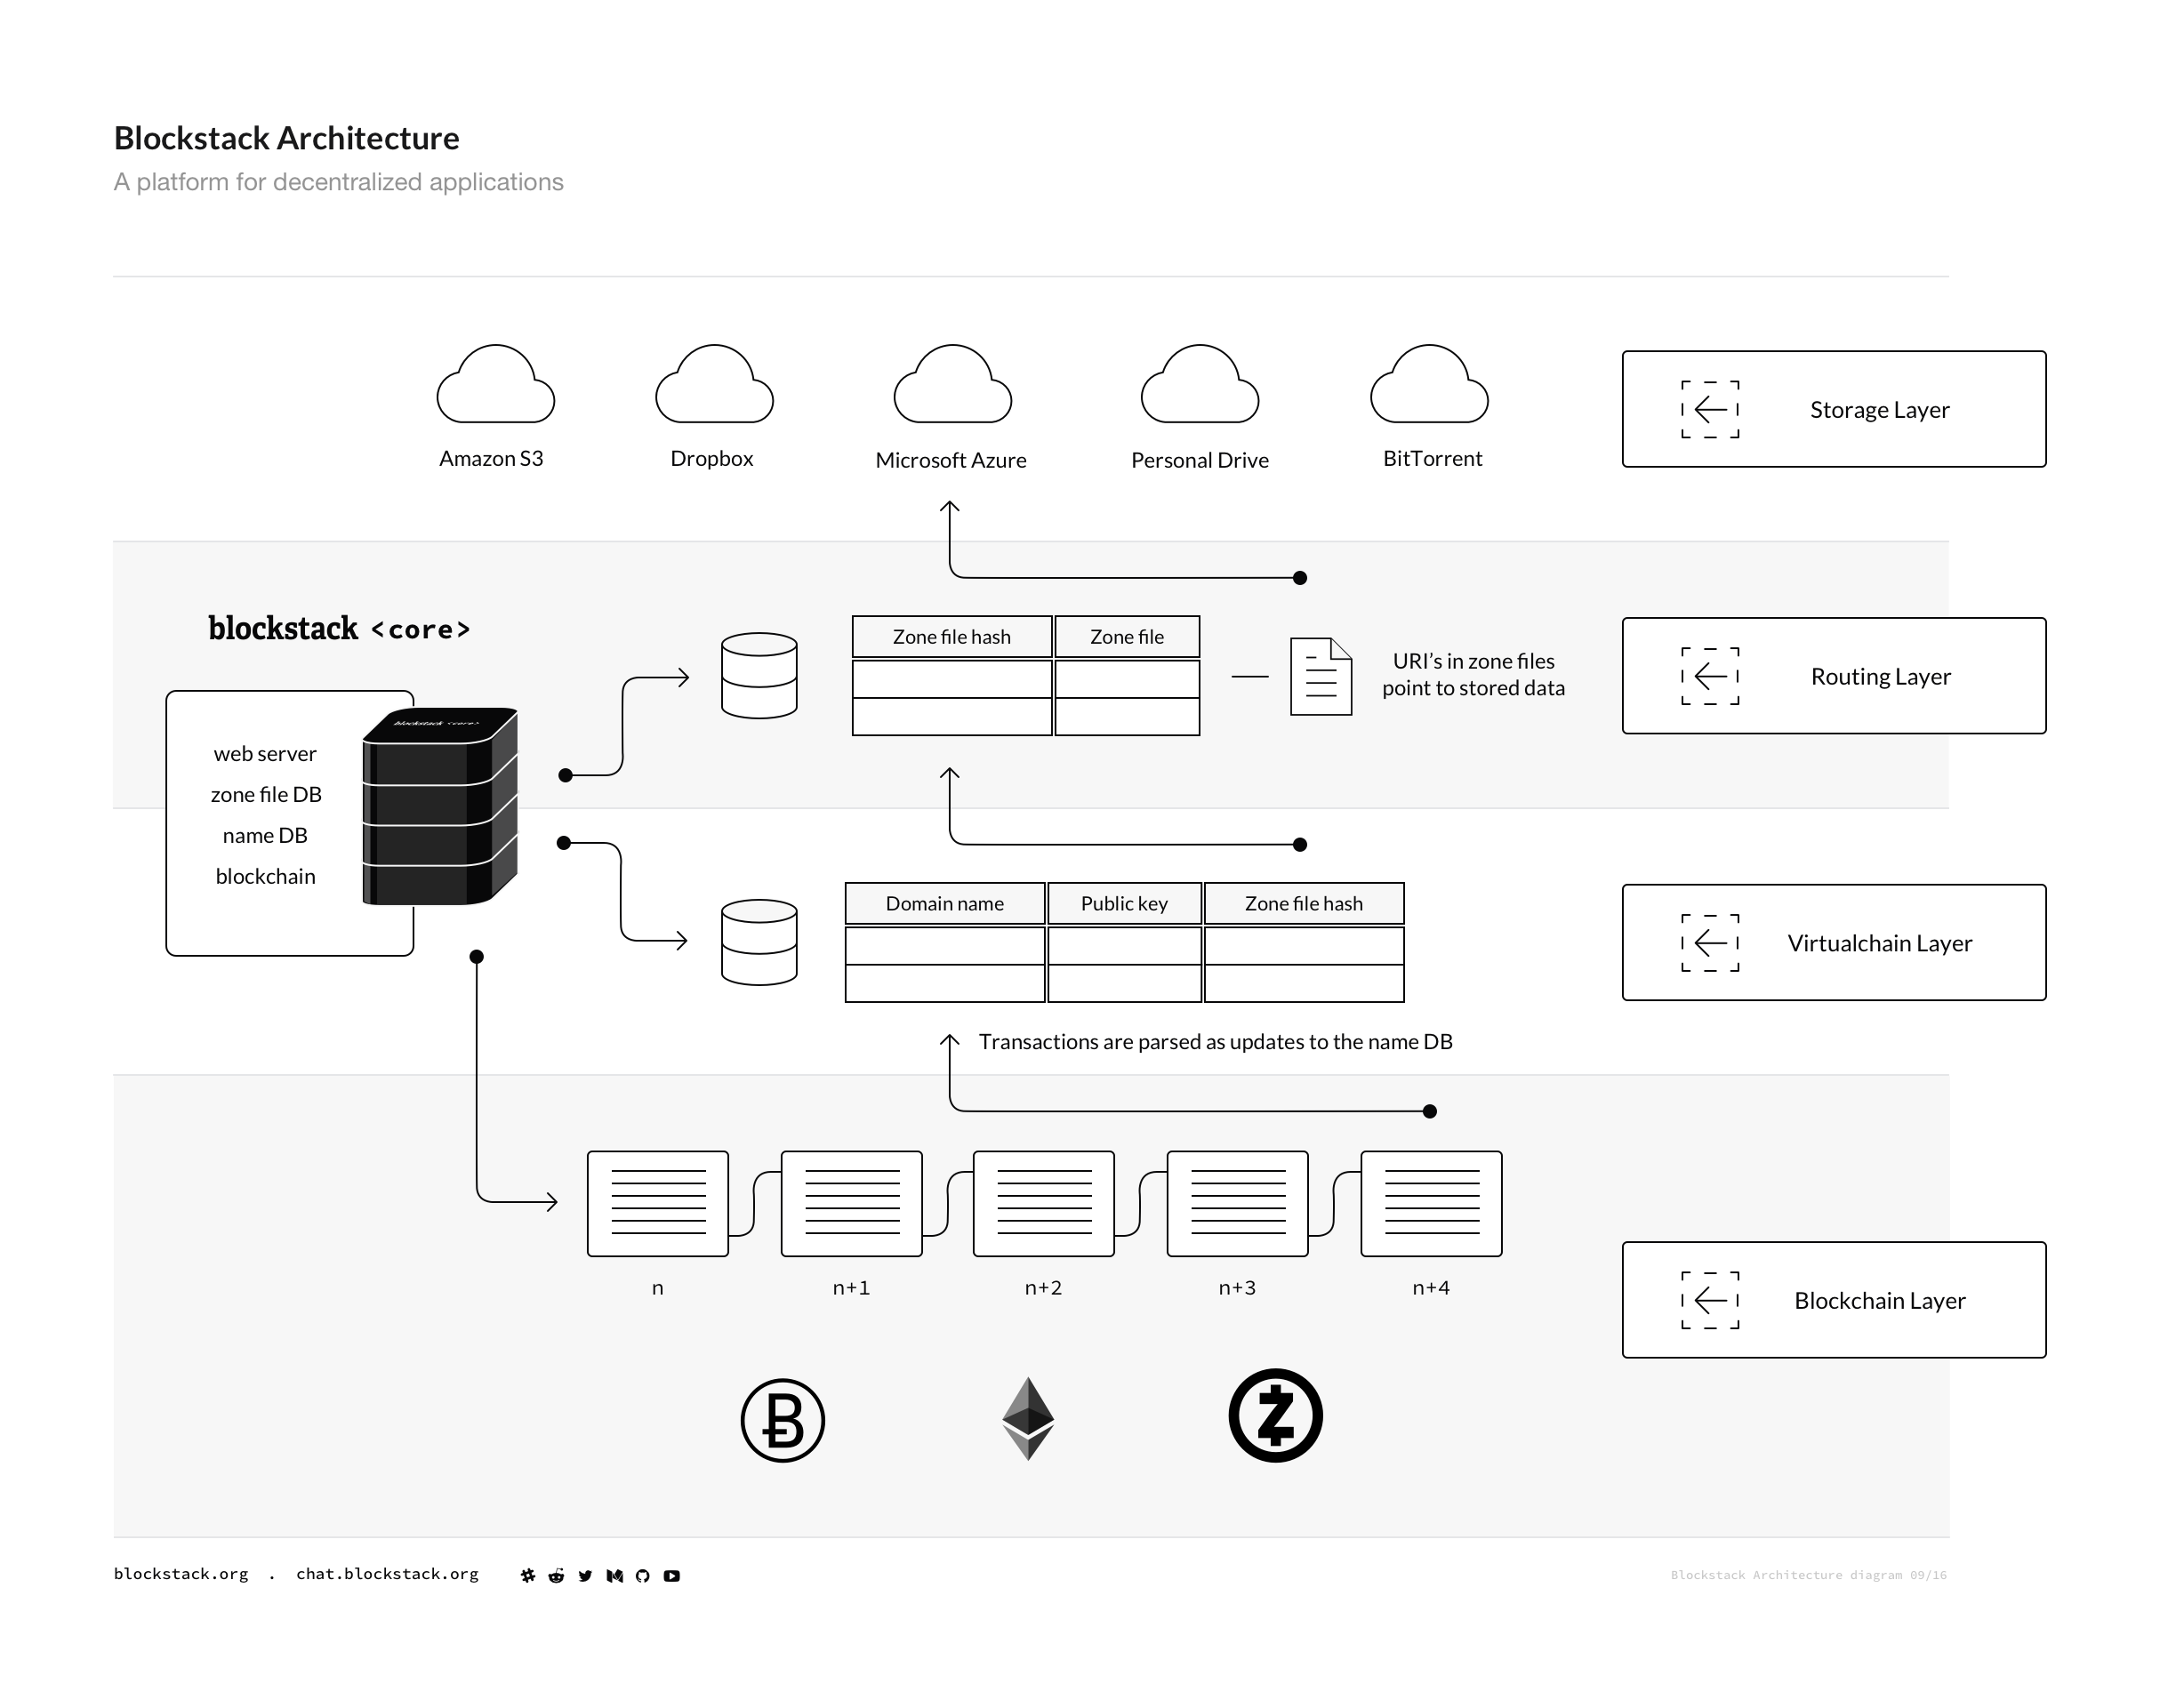
\includegraphics[width=0.8\textwidth]{blockstack-architecture}
	\caption{Basic Blockstack architecture}
	\label{fig1}
\end{figure}

\begin{notation}
	Why did we choose Ethereum
\end{notation}

\section{Solidity}
Solidity is a high level programming language developed specially for Ethereum block chain. Solidity introduced smart contracts which is a base for different use cases like supply chain platforms, Banks, health care system etc. Smart contracts are executed by a computer network that uses consensus protocols to agree upon certain actions resulting from the smart’s contract code. Like other programming languages Solidity support inheritance, user defined types, libraries, control structures, comments and a lot more features. Syntax of solidity language is similar to java script. Due to that reason web developers and programmer can adopt it in very short period of time.

Solidity is still in its early stage while non Ethereum projects are also involved to use solidity. Every language has their own weaknesses while in solidity a lot of things to be improved in near future. Theoretically it’s easy to talk about in idea but in reality it’s impossible to implement every idea in solidity. Solidity was the best fit for our project “identity management in block chain” through which we created contracts for Ethereum block chain.

\subsection{Elliptic Curves}
ECC is the next generation of public key cryptography, and based on currently understood mathematics, it provides a significantly more secure foundation than first-generation public key cryptography systems like RSA.

With ECC, you can use smaller keys to get the same levels of security. Small keys are important, especially in a world where more and more cryptography is done on less powerful devices like mobile phones. While multiplying two prime numbers together is easier than factoring the product into its component parts, when the prime numbers start to get very long, even just the multiplication step can take some time on a low powered device. While you could likely continue to keep RSA secure by increasing the key length, that comes with a cost of slower cryptographic performance on the client. ECC appears to offer a better tradeoff: high security with short, fast keys.

\subsection{RSA}
\begin{notation}
	Write something about RSA?
\end{notation}
